% Guitar chords
% Author: Christoph
% Source: http://rio.eta-ori.net/latex-chords/chords.sty
%         http://rio.eta-ori.net/latex-chords/example.tex
\documentclass{minimal}
\usepackage{tikz}
\usepackage{verbatim}
%\usepackage{subfig}

\usetikzlibrary{arrows, positioning}
\usetikzlibrary{patterns}
\newcommand{\colwidth}{2 cm}

\tikzset{
    %Define standard arrow tip
    >=stealth',
    %Define style for boxes
    punkt/.style={
           rectangle,
           rounded corners,
           draw=black, very thick,
           text width=4em,
           minimum height=2em,
           text centered},
    % Define arrow style
    pil/.style={
           ->,
           very thick,
           shorten <=4pt,
           shorten >=4pt,}
}



\begin{document}

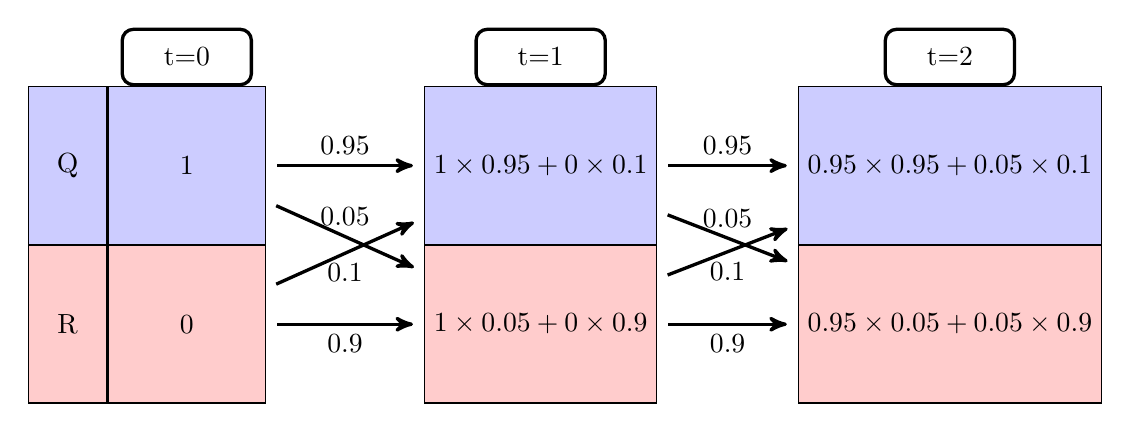
\begin{tikzpicture}[->,node distance=0cm, auto]
%[->,
        %           shorten >=2pt,
       %             auto,
         %           node distance=2cm,
          %          on grid,
         %           very thick,state/.style=state with output,
         %          every state/.style={draw=black!50, very thick, fill=black!20, scale=1},
 %                   x=\colwidth,
  %                  y=1cm, 
            %        node distance=0 cm,
             %       outer sep = 0 cm
   %          ]


% Style for state boxes
\tikzstyle{state1}=[draw, rectangle, minimum height=\colwidth, minimum width=1cm, fill=blue!20,anchor=north east]

\tikzstyle{state2}=[draw, rectangle, minimum height=\colwidth, minimum width=1cm, fill=red!20,anchor=north east]

\tikzstyle{s1t}=[draw, rectangle, minimum height=\colwidth, minimum width=\colwidth, fill=blue!20,anchor=north east]

\tikzstyle{s2t}=[draw, rectangle, minimum height=\colwidth, minimum width=\colwidth, fill=red!20,anchor=north east]


% Styles for events
% Duration of sequences
\tikzstyle{heights}=[rectangle,draw, minimum width=\colwidth, anchor=north west,text centered,text width=5 em]
%\tikzstyle{1height}=[heights,minimum height=1cm]
%\tikzstyle{2heights}=[heights,minimum height=2cm]
%\tikzstyle{3heights}=[heights,minimum height=3cm]
%Style for type of sequence 
%\tikzstyle{Ang2h}=[2heights,fill=green!20]
%\tikzstyle{Phys2h}=[2heights,fill=red!20]
%\tikzstyle{Math2h}=[2heights,fill=blue!20]
%\tikzstyle{TIPE2h}=[2heights,fill=blue!10]
%\tikzstyle{TP2h}=[2heights, pattern=north east lines, pattern color=magenta]
%\tikzstyle{G3h}=[3heights, pattern=north west lines, pattern color=magenta!60!white]
%\tikzstyle{Planche}=[1height,fill=white]
% Positioning labels for days and hours
\node[punkt] (t0) at (1,1) {t=0};
\node[punkt] (t1) [right = 8em of t0] {t=1};
\node[punkt] (t2) [right = 10em of t1] {t=2};
%\node[punkt] (t3) [right = 8em of t2] {t=3};
\node[s1t] (s10) [below = of t0] {1};
\node[s2t] (s20) [below = of s10] {0};
\node[state1] (s1) [left = of s10] {Q};
\node[state2] (s2) [below = of s1] {R};
\node[s1t] (s11) [below = of t1] {$1 \times 0.95+0 \times 0.1$};
\node[s2t] (s21) [below = of s11] {$1 \times 0.05 + 0 \times 0.9$};
\node[s1t] (s12) [below = of t2] {$0.95 \times 0.95+0.05 \times 0.1$};
\node[s2t] (s22) [below = of s12] {$0.95 \times 0.05+0.05 \times 0.9$};
%\node[state2] (s13) [below = of t3] {1};
%\node[state2] (s23) [below = of s13] {0};

\path 
% first set of arrows
(s10) edge[pil] node [above] {0.95} (s11)
(s10) edge[pil] node [above] {0.05} (s21)
(s20) edge[pil] node [below] {0.9} (s21)
(s20) edge[pil] node [below] {0.1} (s11)
% second set of arrows
(s11) edge[pil] node [above] {0.95} (s12)
(s11) edge[pil] node [above] {0.05} (s22)
(s21) edge[pil] node [below] {0.9} (s22)
(s21) edge[pil] node [below] {0.1} (s12);

\end{tikzpicture}


\end{document}
